% FlyTracer: Inside the Framework. Build with: xelatex flytracer-overview.tex (twice, for the contents)
\documentclass[11pt,a4paper]{article}

\usepackage{fontspec}
\setmainfont{Charter}
\setsansfont{Avenir Next}
\setmonofont{Menlo}[Scale=0.82]

\usepackage[a4paper,margin=2.3cm,headheight=14pt]{geometry}
\usepackage[dvipsnames,table]{xcolor}
\usepackage{graphicx}
\usepackage{booktabs}
\usepackage{tabularx}
\usepackage{array}
\usepackage{enumitem}
\usepackage{listings}
\usepackage{tikz}
\usetikzlibrary{arrows.meta,positioning,fit,calc,shapes.misc,backgrounds,patterns}
\usepackage[most]{tcolorbox}
\usepackage{titlesec}
\usepackage{fancyhdr}
\usepackage{caption}
\usepackage[obeyspaces,spaces]{url}
\usepackage[hidelinks]{hyperref}

\definecolor{ink}{HTML}{1F2933}
\definecolor{accent}{HTML}{2563A6}
\definecolor{accentlight}{HTML}{E8F0FA}
\definecolor{warm}{HTML}{B45309}
\definecolor{warmlight}{HTML}{FDF3E4}
\definecolor{green}{HTML}{2F7D4A}
\definecolor{greenlight}{HTML}{E9F5EC}
\definecolor{codebg}{HTML}{F6F7F9}
\definecolor{codeframe}{HTML}{DDE1E6}
\definecolor{comment}{HTML}{6B7785}
\definecolor{keyword}{HTML}{8A3FB0}
\definecolor{string}{HTML}{2F7D4A}
\definecolor{muted}{HTML}{5B6573}

\color{ink}
\setlength{\parindent}{0pt}
\setlength{\parskip}{6pt}
\setlength{\emergencystretch}{2.5em}
\linespread{1.08}

\titleformat{\section}{\sffamily\Large\bfseries\color{accent}}{\thesection}{0.7em}{}
\titleformat{\subsection}{\sffamily\large\bfseries}{\thesubsection}{0.7em}{}
\titleformat{\subsubsection}{\sffamily\normalsize\bfseries}{}{0em}{}
\titlespacing*{\section}{0pt}{18pt}{6pt}
\titlespacing*{\subsection}{0pt}{12pt}{3pt}
\titlespacing*{\subsubsection}{0pt}{8pt}{0pt}

\newcommand{\partheading}[2]{%
  \clearpage
  \begin{tikzpicture}[remember picture,overlay]
    \fill[accent] (current page.north west) rectangle ([yshift=-0.9cm]current page.north east);
  \end{tikzpicture}
  \vspace*{0.4cm}
  {\sffamily\small\bfseries\color{accent} PART #1}\par\vspace{-4pt}
  {\sffamily\huge\bfseries #2}\par\vspace{6pt}
  \addcontentsline{toc}{part}{Part #1\quad #2}}

\pagestyle{fancy}
\fancyhf{}
\fancyhead[L]{\sffamily\footnotesize\color{muted} FlyTracer: Inside the Framework}
\fancyhead[R]{\sffamily\footnotesize\color{muted}\nouppercase{\leftmark}}
\fancyfoot[C]{\sffamily\footnotesize\color{muted}\thepage}
\renewcommand{\headrulewidth}{0.3pt}
\renewcommand{\sectionmark}[1]{\markboth{#1}{}}

\captionsetup{font={small,sf},labelfont=bf,justification=raggedright,singlelinecheck=false}

% Inline code that may break at underscores and dots
\DeclareUrlCommand\code{\urlstyle{tt}}
\renewcommand{\UrlBreaks}{\do\_\do.\do:\do/}

\lstdefinestyle{base}{
  basicstyle=\ttfamily\footnotesize,
  backgroundcolor=\color{codebg},
  frame=single, rulecolor=\color{codeframe}, framesep=6pt, xleftmargin=6pt, xrightmargin=6pt,
  commentstyle=\color{comment}\itshape,
  keywordstyle=\color{keyword}\bfseries,
  stringstyle=\color{string},
  showstringspaces=false, columns=fullflexible, keepspaces=true,
  breaklines=true, breakatwhitespace=true,
  aboveskip=8pt, belowskip=6pt, tabsize=4,
  upquote=true,
}
\lstdefinestyle{cpp}{style=base, language=C++,
  morekeywords={constexpr,noexcept,nullptr,override,final,auto,decltype,consteval,requires,concept,co_await,static_assert,inline,using,template,typename},
  literate={~}{{\textasciitilde}}1}
\lstdefinestyle{glsl}{style=base, language=C,
  morekeywords={layout,uniform,buffer,readonly,writeonly,in,out,inout,vec2,vec3,vec4,ivec2,uint,image2D,sampler2D,binding,push_constant,scalar,rgba32f,rgba8,local_size_x,local_size_y}}
\lstdefinestyle{shell}{style=base, language=bash}
\lstset{style=cpp}

\newtcolorbox{keyidea}[1][Key idea]{enhanced, breakable, colback=accentlight, colframe=accent,
  boxrule=0pt, leftrule=3pt, arc=0pt, left=8pt, right=8pt, top=4pt, bottom=4pt,
  fonttitle=\sffamily\bfseries\small, coltitle=accent, colbacktitle=accentlight,
  title={#1}, attach title to upper={\par\vspace{2pt}}}
\newtcolorbox{pitfall}[1][Pitfall]{enhanced, breakable, colback=warmlight, colframe=warm,
  boxrule=0pt, leftrule=3pt, arc=0pt, left=8pt, right=8pt, top=4pt, bottom=4pt,
  fonttitle=\sffamily\bfseries\small, coltitle=warm, colbacktitle=warmlight,
  title={#1}, attach title to upper={\par\vspace{2pt}}}
\newtcolorbox{tryit}[1][Try it]{enhanced, breakable, colback=greenlight, colframe=green,
  boxrule=0pt, leftrule=3pt, arc=0pt, left=8pt, right=8pt, top=4pt, bottom=4pt,
  fonttitle=\sffamily\bfseries\small, coltitle=green, colbacktitle=greenlight,
  title={#1}, attach title to upper={\par\vspace{2pt}}}

\DeclareUrlCommand\file{\def\UrlFont{\sffamily\small\color{accent}}}

\tikzset{
  box/.style={draw=accent, fill=white, rounded corners=2pt, align=center, font=\sffamily\small,
              minimum height=0.9cm, inner sep=5pt},
  fillbox/.style={box, fill=accentlight},
  warmbox/.style={box, draw=warm, fill=warmlight},
  greenbox/.style={box, draw=green, fill=greenlight},
  arrow/.style={-{Stealth[length=2.2mm]}, thick, color=muted},
  label/.style={font=\sffamily\scriptsize, color=muted, align=center},
}

\setlist{itemsep=2pt, topsep=2pt, parsep=2pt}

\begin{document}

% ---------------------------------------------------------------- Title page
\begin{titlepage}
\begin{tikzpicture}[remember picture,overlay]
  \fill[accent] (current page.north west) rectangle ([yshift=-7.2cm]current page.north east);
  \node[anchor=north west, text=white, align=left, inner sep=0] at ([xshift=2.3cm,yshift=-2.2cm]current page.north west)
    {\sffamily\small\bfseries DAE \textbullet{} GEOMETRIC ALGEBRA};
  \node[anchor=north west, text=white, align=left, inner sep=0] at ([xshift=2.3cm,yshift=-2.9cm]current page.north west)
    {\sffamily\fontsize{38}{40}\selectfont\bfseries FlyTracer};
  \node[anchor=north west, text=white, align=left, inner sep=0] at ([xshift=2.3cm,yshift=-4.5cm]current page.north west)
    {\sffamily\LARGE Inside the Framework};
  \node[anchor=north west, text=white!85!accent, align=left, inner sep=0, text width=15cm] at ([xshift=2.3cm,yshift=-5.6cm]current page.north west)
    {\sffamily\normalsize How a real-time PGA raytracer is put together, from the game loop to the last Vulkan barrier};
\end{tikzpicture}
\vspace*{6.2cm}

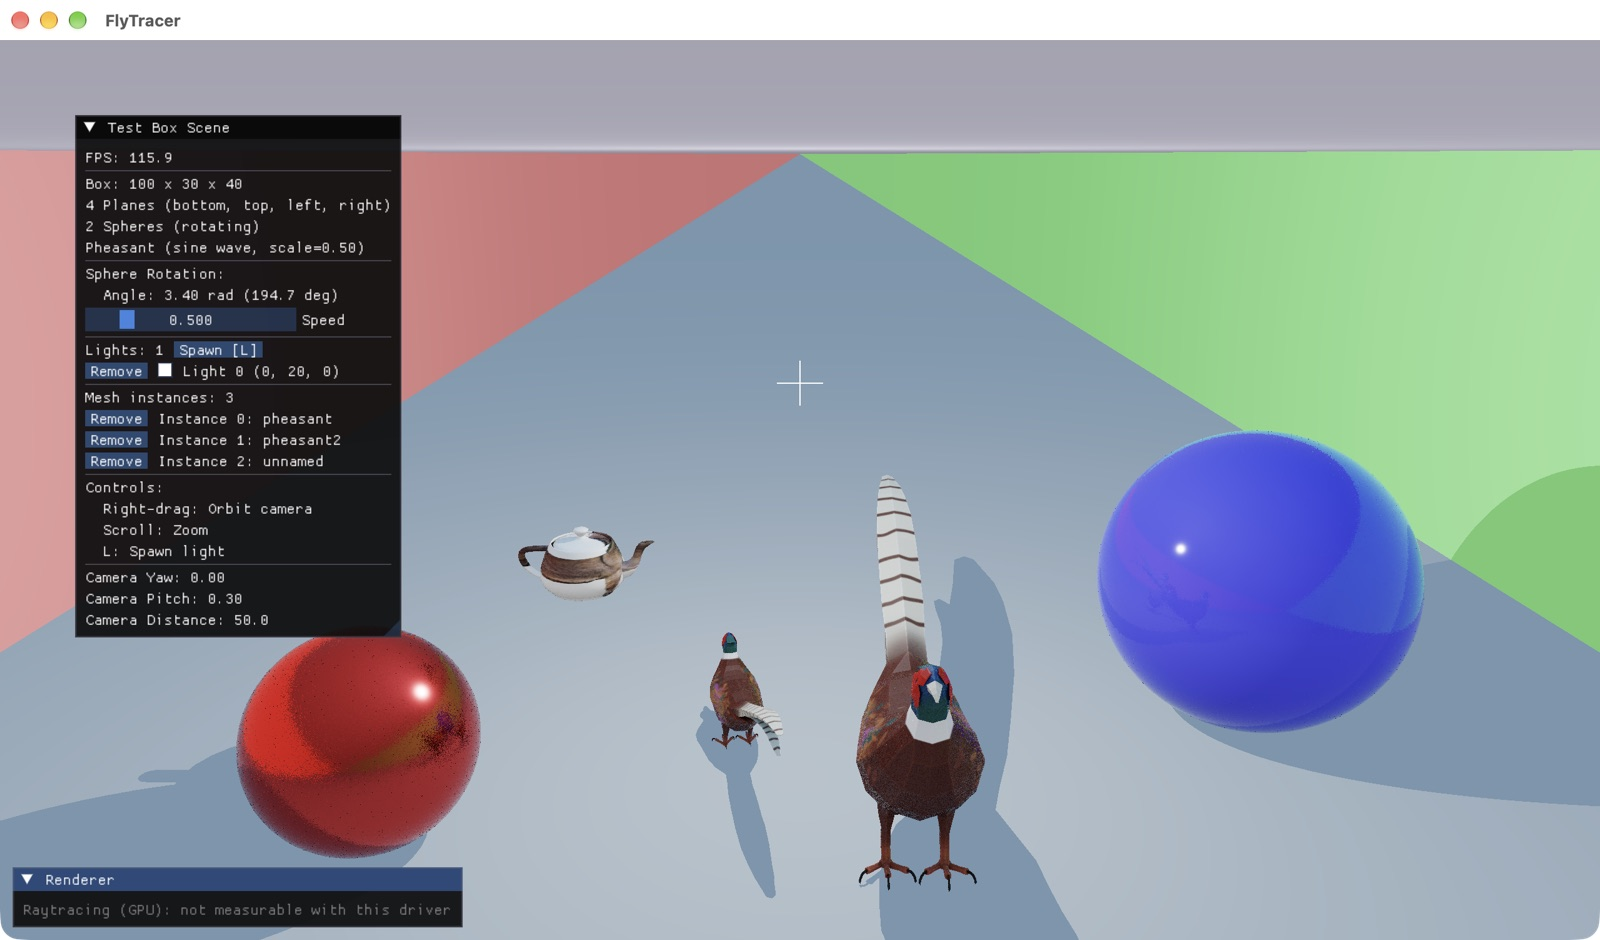
\includegraphics[width=\textwidth]{images/testbox.jpg}

{\sffamily\footnotesize\color{muted} The \code{testbox} scene: planes, spheres and textured meshes, raytraced every frame in one compute shader, with the Dear ImGui panels drawn on top.}

\vfill
\begin{minipage}[t]{0.48\textwidth}
\sffamily\small
\textbf{What you will learn}\par\smallskip
\begin{itemize}[leftmargin=1.2em]
  \item How the engine, the game and the shader divide the work
  \item How a scene becomes bytes in GPU buffers
  \item Every Vulkan object FlyTracer creates, and why
  \item How one frame is recorded, synchronized and presented
\end{itemize}
\end{minipage}\hfill
\begin{minipage}[t]{0.48\textwidth}
\sffamily\small
\textbf{What you should know already}\par\smallskip
\begin{itemize}[leftmargin=1.2em]
  \item C++ (classes, RAII, lambdas, \code{std::vector})
  \item The PGA basics: points, planes, lines, motors
  \item What a raytracer does, roughly
\end{itemize}
No Vulkan experience is needed: Part II introduces every concept as it appears in the code.
\end{minipage}

\vspace{1cm}
{\sffamily\footnotesize\color{muted} Version of October 2026. Code excerpts are taken from the repository and sometimes shortened; ``\code{// ...}'' marks a cut.}
\end{titlepage}

\tableofcontents
\clearpage

% ================================================================= PART I
\partheading{I}{The Framework}

\section{What FlyTracer is}

FlyTracer is a real-time raytracer written to teach Projective Geometric Algebra (PGA). Everything that moves (the camera, mesh instances, reflections) is a PGA element: points are \code{TriVector}s, planes are \code{Vector}s, lines are \code{BiVector}s and rigid motions are \code{Motor}s, all from the header-only FlyFish library. There are no matrices, not on the CPU and not on the GPU.

The image is computed by a single Vulkan compute shader, \file{engine/shaders/raytracer.comp}. Every frame it shoots one ray per pixel, follows reflections, adds the result to a running average and writes a finished image that is copied to the window. The C++ side prepares the scene, uploads it, and orchestrates the GPU work.

\begin{figure}[h]
\centering
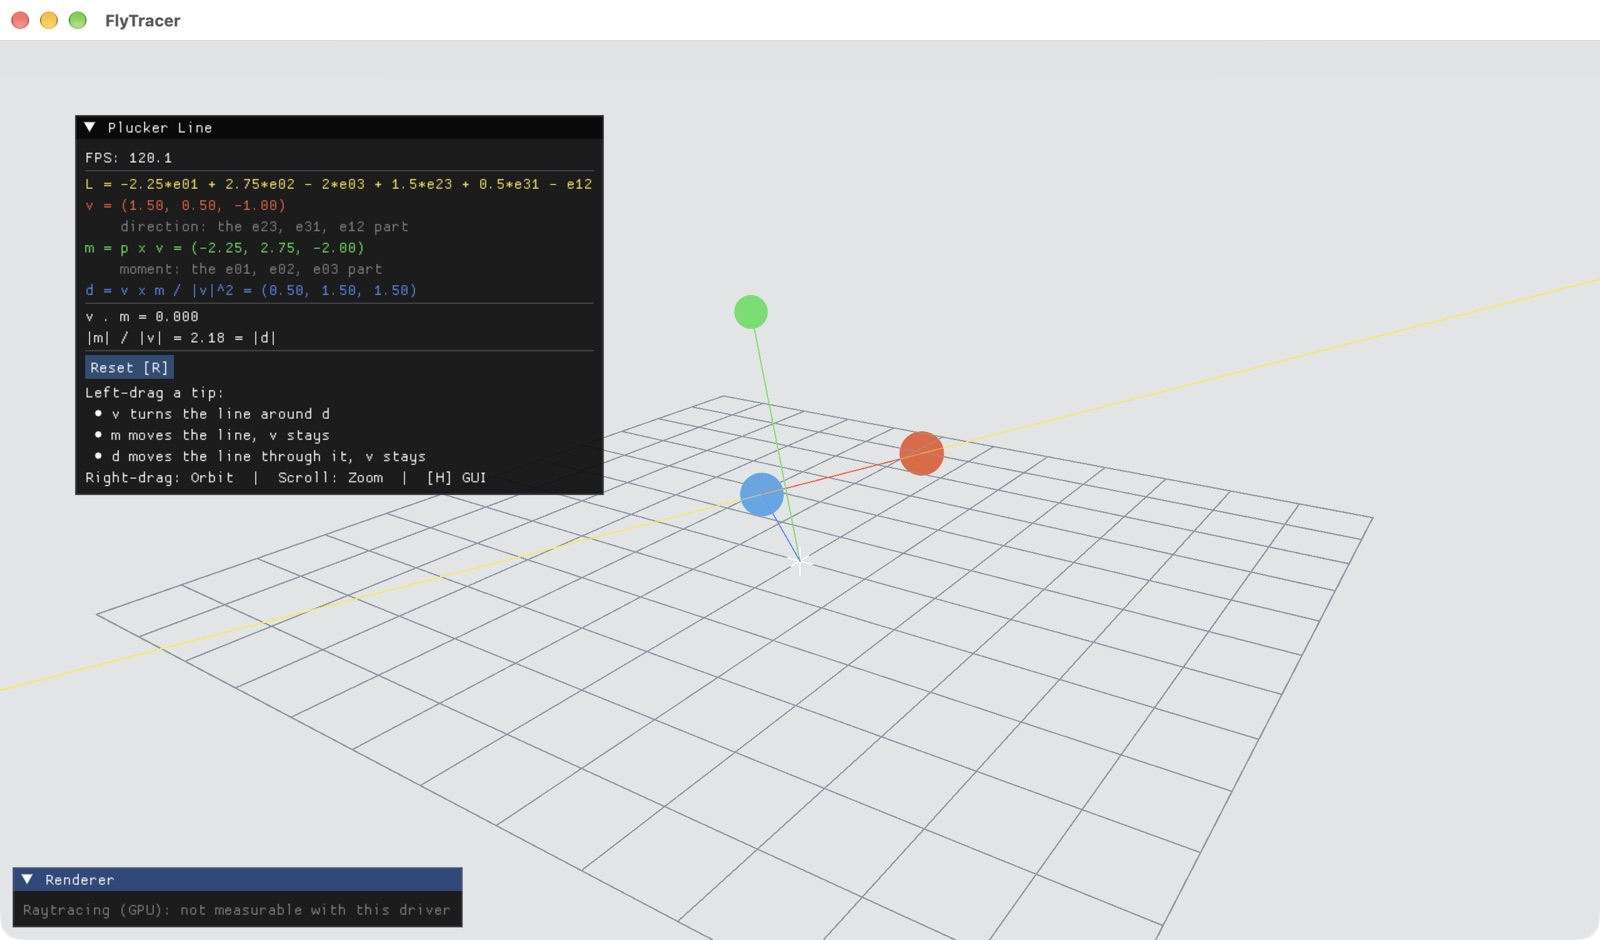
\includegraphics[width=0.49\textwidth]{images/plucker.jpg}\hfill
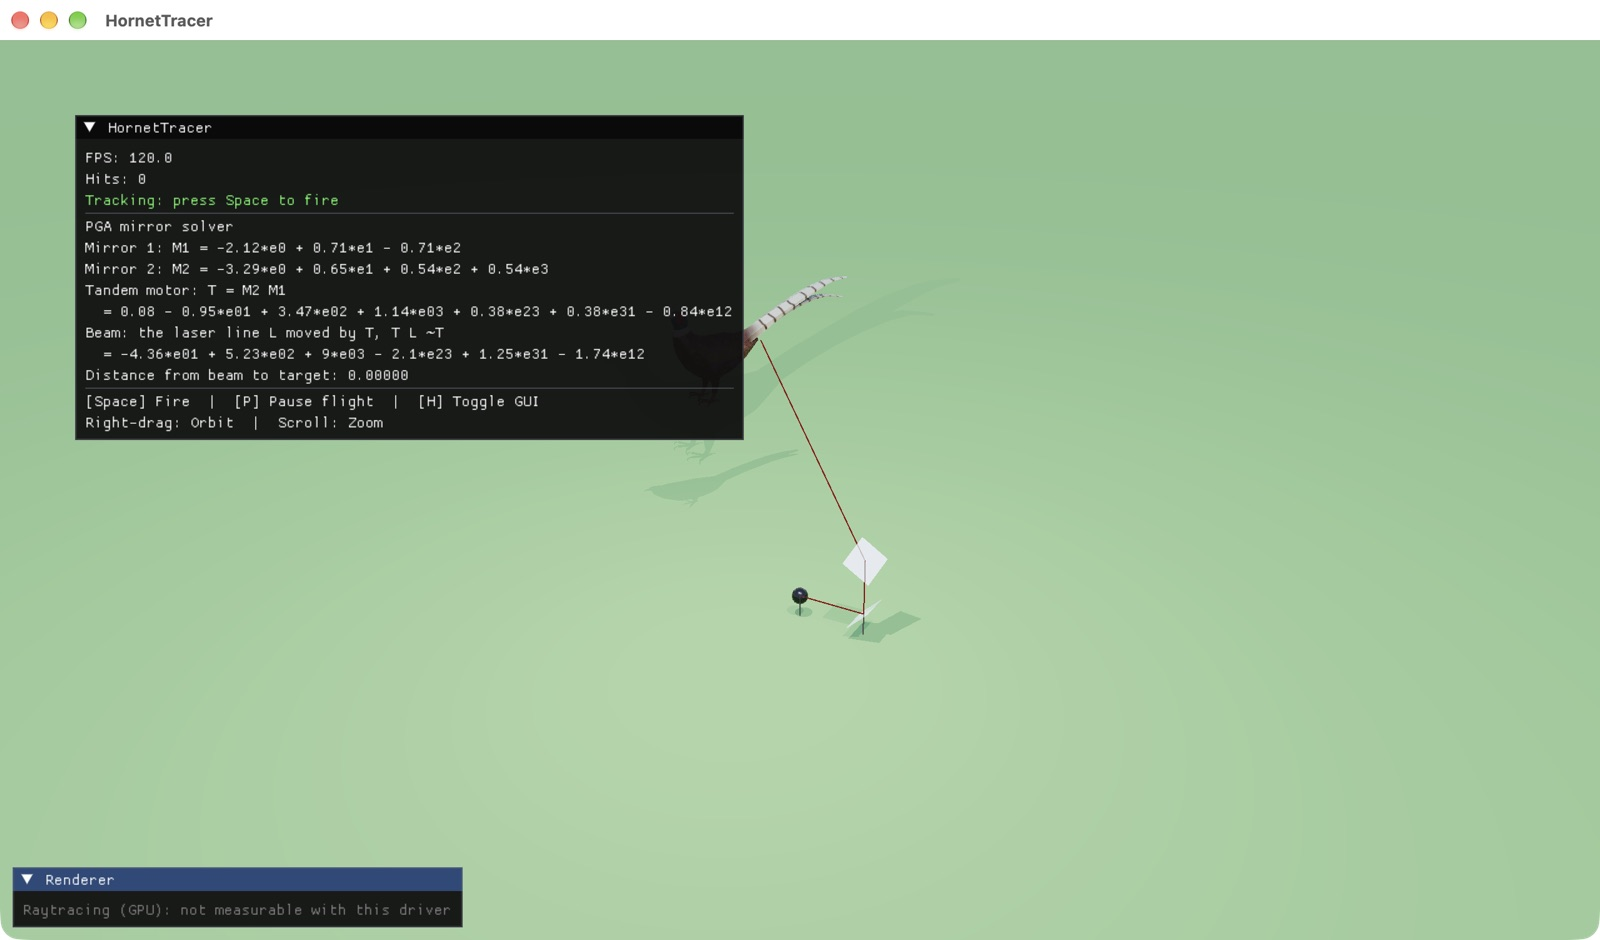
\includegraphics[width=0.49\textwidth]{images/hornet.jpg}
\caption{Two of the teaching scenes. Left: \texttt{plucker}, a line in Plücker coordinates with its direction, moment and support vector as debug lines. Right: \texttt{hornet}, two mirrors solved with PGA steer a laser beam onto a target.}
\end{figure}

\subsection{How to read this document}

\begin{description}[font=\sffamily\bfseries, leftmargin=0pt, itemsep=4pt]
  \item[Part I, the framework] follows one frame through the C++ code: the main loop, the scene API that students program against, and how the scene is encoded into GPU structs.
  \item[Part II, the Vulkan code] explains every Vulkan object FlyTracer creates, in the order they are created, and then the synchronization of a frame in detail.
  \item[Part III, the GPU] walks through the compute shader and ends with testing, debugging and exercises.
\end{description}

Coloured boxes mark \textcolor{accent}{\textbf{key ideas}}, \textcolor{warm}{\textbf{pitfalls}} and \textcolor{green}{\textbf{things to try}}.

\subsection{Where things live}

\begin{center}
\small
\begin{tabularx}{\textwidth}{@{}>{\sffamily}l X@{}}
\toprule
\textbf{Path} & \textbf{Contents} \\
\midrule
\file{engine/include}, \file{engine/src} & The engine: two static libraries, \code{FlyTracerCore} and \code{FlyTracerEngine} \\
\file{engine/shaders} & The GLSL compute shader and its include files, compiled to SPIR-V by \code{glslc} \\
\file{game/} & The executable: \code{main.cpp}, the scene registry and the teaching scenes \\
\file{game/resources} & OBJ meshes and textures, copied next to the executable \\
\file{tests/} & Google Test unit tests, GPU tests and golden reference images \\
\file{docs/} & The student documentation (MkDocs) and this overview \\
\bottomrule
\end{tabularx}
\end{center}

\begin{lstlisting}[style=shell]
cmake -B build -DCMAKE_BUILD_TYPE=Release   # Debug enables the validation layer
cmake --build build                          # executable, shaders, resources and tests
./build/bin/FlyTracer --scene testbox        # also debug, bireflection, birot, plucker, ...
ctest --test-dir build
\end{lstlisting}

% -----------------------------------------------------------------
\section{Architecture}

FlyTracer is split into layers that only depend downwards (Figure~\ref{fig:layers}). The split is not cosmetic: each boundary is something you can test or replace on its own.

\begin{figure}[h]
\centering
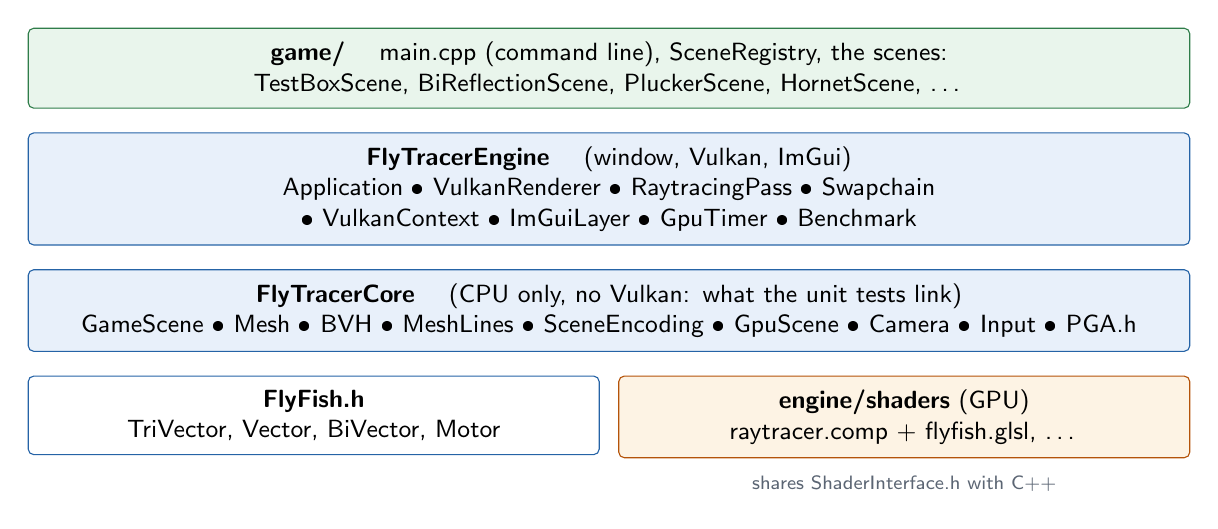
\begin{tikzpicture}[node distance=3mm]
  \node[greenbox, text width=14.4cm] (game) {\textbf{game/} \quad \code{main.cpp} (command line), \code{SceneRegistry}, the scenes:\\ \code{TestBoxScene}, \code{BiReflectionScene}, \code{PluckerScene}, \code{HornetScene}, \dots};
  \node[fillbox, text width=14.4cm, below=of game] (engine) {\textbf{FlyTracerEngine} \quad (window, Vulkan, ImGui)\\ \code{Application} \textbullet{} \code{VulkanRenderer} \textbullet{} \code{RaytracingPass} \textbullet{} \code{Swapchain} \textbullet{} \code{VulkanContext} \textbullet{} \code{ImGuiLayer} \textbullet{} \code{GpuTimer} \textbullet{} \code{Benchmark}};
  \node[fillbox, text width=14.4cm, below=of engine] (core) {\textbf{FlyTracerCore} \quad (CPU only, no Vulkan: what the unit tests link)\\ \code{GameScene} \textbullet{} \code{Mesh} \textbullet{} \code{BVH} \textbullet{} \code{MeshLines} \textbullet{} \code{SceneEncoding} \textbullet{} \code{GpuScene} \textbullet{} \code{Camera} \textbullet{} \code{Input} \textbullet{} \code{PGA.h}};
  \node[box, text width=6.9cm, below=of core.south west, anchor=north west] (flyfish) {\textbf{FlyFish.h}\\ \code{TriVector}, \code{Vector}, \code{BiVector}, \code{Motor}};
  \node[warmbox, text width=6.9cm, below=of core.south east, anchor=north east] (shader) {\textbf{engine/shaders} (GPU)\\ \code{raytracer.comp} + \code{flyfish.glsl}, \dots};
  \node[label, below=1mm of shader] {shares \code{ShaderInterface.h} with C++};
\end{tikzpicture}
\caption{The layers. Each one only uses the layers below it.}
\label{fig:layers}
\end{figure}

\begin{description}[font=\sffamily\bfseries, leftmargin=0pt]
  \item[FlyTracerCore] knows the scene: meshes, bounding volume hierarchies, the camera, and how all of it is laid out in bytes for the GPU. It never includes \code{vulkan.h}, so \code{FlyTracer_Test} runs on any machine, also without a GPU.
  \item[FlyTracerEngine] owns the window and everything Vulkan. It only reads the scene through the const getters of \code{GameScene}.
  \item[The game] contains no engine code at all: a scene derives from \code{GameScene} and uses its protected API.
  \item[The shader] is a separate program. The contract between it and C++ is \file{ShaderInterface.h} (binding numbers and limits, \code{#define}s both languages include) and the structs in \file{GpuScene.h}, which a GPU test checks against the GLSL structs.
\end{description}

\subsection{Who owns what}

Ownership follows the RAII idiom: an object's members are constructed in declaration order and destroyed in reverse. FlyTracer uses this deliberately. \code{VulkanRenderer} declares the context first, so it is destroyed last, after everything that was created from it:

\begin{lstlisting}
class VulkanRenderer {
    // ...
    SDL_Window* m_window;
    // Declaration order is construction order; destruction runs backwards, so the context goes last
    VulkanContext m_context;
    Swapchain m_swapchain;
    RaytracingPass m_raytracing;
    ImGuiLayer m_imgui;
    std::array<Frame, RaytracingPass::kFramesInFlight> m_frames;
    // ...
};
\end{lstlisting}

\code{Application} owns the SDL window, the \code{VulkanRenderer}, the \code{GameScene} and the \code{Input} state. There are no global objects and no singletons.

% -----------------------------------------------------------------
\section{One frame, from the top}

The whole program is a loop in \code{Application::run} (\file{engine/src/Application.cpp}):

\begin{lstlisting}
while (m_running) {
    const double deltaTime = std::min(/* seconds since the last frame */, kMaxDeltaTime);
    handleEvents();                          // SDL events -> Input (keys, mouse, resize, quit)
    // ...
    m_gameScene->HandleInput(m_input);       // the scene reacts to input
    m_input.EndFrame();
    m_gameScene->Update(static_cast<float>(deltaTime));   // the scene animates
    render(static_cast<float>(deltaTime));
}
m_renderer->WaitIdle();

void Application::render(float deltaTime) {
    if (!m_renderer->BeginFrame()) return;   // no image available (minimized, resizing)
    m_gameScene->DrawGui();                  // ImGui windows of the scene
    drawRendererStats(deltaTime);
    m_renderer->EndFrame(*m_gameScene);      // record, submit and present
}
\end{lstlisting}

\begin{figure}[h]
\centering
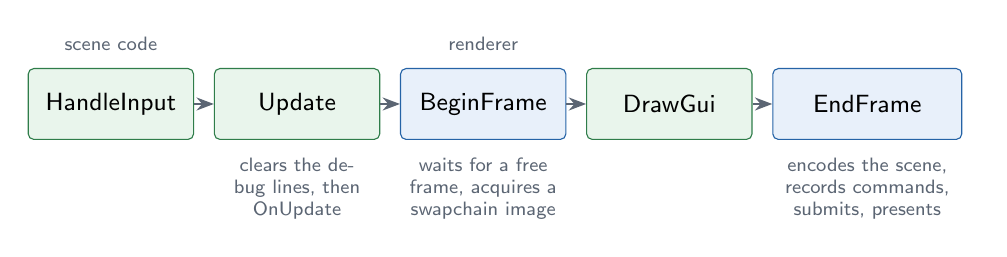
\begin{tikzpicture}[node distance=2.5mm and 2.5mm, every node/.style={font=\sffamily\scriptsize}]
  \node[greenbox, minimum width=2.1cm] (in) {HandleInput};
  \node[greenbox, minimum width=2.1cm, right=of in] (up) {Update};
  \node[fillbox, minimum width=2.1cm, right=of up] (bf) {BeginFrame};
  \node[greenbox, minimum width=2.1cm, right=of bf] (gui) {DrawGui};
  \node[fillbox, minimum width=2.4cm, right=of gui] (ef) {EndFrame};
  \draw[arrow] (in) -- (up); \draw[arrow] (up) -- (bf); \draw[arrow] (bf) -- (gui); \draw[arrow] (gui) -- (ef);
  \node[label, below=1mm of up, text width=2.3cm] {clears the debug lines, then \code{OnUpdate}};
  \node[label, below=1mm of bf, text width=2.4cm] {waits for a free frame, acquires a swapchain image};
  \node[label, below=1mm of ef, text width=2.6cm] {encodes the scene, records commands, submits, presents};
  \node[label, above=1mm of in] {scene code};
  \node[label, above=1mm of bf] {renderer};
\end{tikzpicture}
\caption{The steps of one frame. Green steps call into the scene, blue ones are the renderer.}
\end{figure}

Two details are worth noticing. First, \code{deltaTime} is clamped, so a frame that took very long (a breakpoint, dragging the window) does not make animations jump. Second, ImGui's frame is opened in \code{BeginFrame} and closed in \code{EndFrame}; \code{DrawGui} sits in between so scenes can create windows with plain \code{ImGui::Begin}.

% -----------------------------------------------------------------
\section{Writing a scene: the GameScene API}

\subsection{Non-virtual interface}

\code{GameScene} (\file{engine/include/GameScene.h}) uses the \emph{non-virtual interface} idiom: the engine calls public, non-virtual functions, which call protected virtual hooks that scenes override.

\begin{center}
\small
\begin{tabular}{@{}lll@{}}
\toprule
\textbf{Engine calls} & \textbf{Scene overrides} & \textbf{What the wrapper adds} \\
\midrule
\code{Init()} & \code{OnInit()} & \\
\code{HandleInput(input)} & \code{OnInput(input)} & \\
\code{Update(dt)} & \code{OnUpdate(dt)} & FPS counter; clears last frame's debug lines \\
\code{DrawGui()} & \code{OnGui()} & \\
\code{Shutdown()} & \code{OnShutdown()} & \\
\bottomrule
\end{tabular}
\end{center}

The wrapper guarantees an order a scene cannot forget: debug lines are always cleared before \code{OnUpdate}, so a scene simply draws the lines it wants this frame.

\subsection{Meshes, instances and primitives}

A \emph{mesh} is geometry loaded once (\code{LoadMesh("pheasant.obj", "pheasant.png")} or \code{AddMesh} for one built in code); its bottom-level BVH is built when it is added. An \emph{instance} places a mesh in the world. Many instances can share one mesh, which is why the two pheasants in \code{testbox} cost almost nothing extra.

\begin{lstlisting}
struct MeshInstance {
    uint32_t meshId{0};
    Motor transform{1.0f, 0.0f, 0.0f, 0.0f, 0.0f, 0.0f, 0.0f, 0.0f};
    float scale{1.0f};
    std::optional<Vector> mirror;   // a reflection after the motor: an odd versor
    bool visible{true};
    std::string name;
};
\end{lstlisting}

A local point $p$ goes to $M\,(s\,p)\,\widetilde{M}$, followed by the reflection in the mirror plane when there is one. Spheres, planes and lights are analytic primitives, added with \code{AddSphere}, \code{AddPlane} and \code{AddPointLight} and friends. All \code{Add*} functions return an id that stays valid when other objects are removed.

\subsection{An example}

This is most of \file{game/src/TestBoxScene.cpp}. Note that animation is pure PGA: a motor is built from an angle and a line, and applied with a sandwich.

\begin{lstlisting}
void TestBoxScene::OnInit() {
    AddPlane(Vector(0.0f, 0.0f, 1.0f, 0.0f), Scene::Material::Lambert(Scene::Color(0.6f, 0.6f, 0.6f)));
    // ... three more planes
    m_sphere1Id = AddSphere(TriVector(m_sphere1Radius, m_sphere1Height, 0.0f), 5.0f,
                            Scene::Material::Metal(Scene::Color(0.9f, 0.3f, 0.3f), 0.2f));
    m_pheasantMeshId = LoadMesh("pheasant.obj", "pheasant.png");
    AddMeshInstance(m_pheasantMeshId, TriVector(0.0f, m_pheasantHeight, 0.0f), "pheasant");
    AddPointLight(TriVector(0.0f, 20.0f, 0.0f), Scene::Color(1.0f, 1.0f, 1.0f), 2.0f, 100.0f);
}

void TestBoxScene::OnUpdate(float deltaTime) {
    m_rotationAngle = std::fmod(m_rotationAngle + m_rotationSpeed * deltaTime, 2.0f * kPi);
    const Motor rotation = Motor::Rotation(m_rotationAngle * RAD_TO_DEG,
                                           BiVector(0.0f, 0.0f, 0.0f, 0.0f, 1.0f, 0.0f));
    if (auto* sphere = GetSphere(m_sphere1Id)) {
        sphere->center = ApplyMotor(rotation, TriVector(m_sphere1Radius, m_sphere1Height, 0.0f));
    }
    if (auto* pheasant = FindInstance("pheasant")) {
        const float sway = m_pheasantSway * std::sin(m_pheasantTime);
        pheasant->transform = rotation * TranslationMotor(sway, m_pheasantHeight, 0.0f);
    }
}

void TestBoxScene::OnInput(const Input& input) {
    m_orbit.HandleInput(input);                  // right-drag orbit, scroll zoom
    SetCamera(m_orbit.Eye(), m_orbit.target);
}
\end{lstlisting}

\begin{pitfall}[Pitfall: motor order]
\code{A * B} applies \code{B} first. \code{rotation * TranslationMotor(...)} translates the pheasant and then rotates the result about the y-axis, so it swings around the origin. Swap the factors and it turns on the spot at its new position instead.
\end{pitfall}

\begin{tryit}[Try it: add a scene]
Create \file{game/include/MyScene.h} and \file{game/src/MyScene.cpp} deriving from \code{GameScene}, add the \code{.cpp} to the executable in \file{CMakeLists.txt}, and register the name in \file{game/src/SceneRegistry.cpp}. Run it with \code{--scene <name>}. The scene test will record a reference image for it the first time it runs.
\end{tryit}

% -----------------------------------------------------------------
\section{From scene to bytes}
\label{sec:encoding}

The GPU cannot read a \code{std::vector<std::unique_ptr<Mesh>>}. Before each frame the scene is \emph{encoded}: flattened into arrays of plain structs whose memory layout matches the GLSL structs byte for byte. This happens entirely in \code{FlyTracerCore} (\file{SceneEncoding.h}, \file{GpuScene.h}), so it is unit-tested without a GPU.

\begin{figure}[h]
\centering
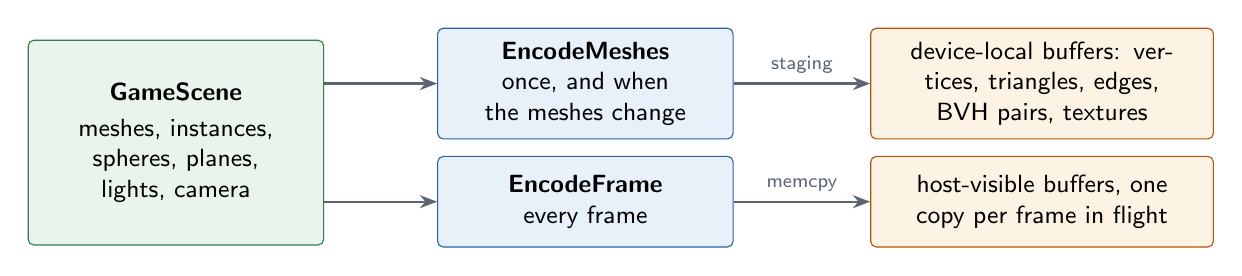
\begin{tikzpicture}[every node/.style={font=\sffamily\small}]
  \node[greenbox, text width=3.4cm, minimum height=2.6cm] (scene) at (0, 0) {\textbf{GameScene}\\[2pt] meshes, instances, spheres, planes, lights, camera};
  \node[fillbox, text width=3.4cm, minimum height=1.15cm] (meshes) at (5.2, 0.75) {\textbf{EncodeMeshes}\\ once, and when the meshes change};
  \node[fillbox, text width=3.4cm, minimum height=1.15cm] (frame) at (5.2, -0.75) {\textbf{EncodeFrame}\\ every frame};
  \node[warmbox, text width=4.0cm, minimum height=1.15cm] (static) at (11.0, 0.75) {device-local buffers: vertices, triangles, edges, BVH pairs, textures};
  \node[warmbox, text width=4.0cm, minimum height=1.15cm] (dyn) at (11.0, -0.75) {host-visible buffers, one copy per frame in flight};
  \draw[arrow] (scene.east |- meshes) -- (meshes.west);
  \draw[arrow] (scene.east |- frame) -- (frame.west);
  \draw[arrow] (meshes) -- node[label, above] {staging} (static);
  \draw[arrow] (frame) -- node[label, above] {memcpy} (dyn);
\end{tikzpicture}
\caption{Two kinds of encoding. Geometry rarely changes, so it lives in fast device-local memory. Everything else is small and is rewritten every frame.}
\end{figure}

\subsection{GPU structs}

Each scene type has a \code{Gpu::} twin and an \code{Encode} function that converts it: colours go from sRGB to linear, planes and motors are normalized, a motor is split into a rotor part and a dual part of four floats each.

\begin{lstlisting}
namespace Gpu {
struct Sphere {
    Float3 center;          // std::array<float, 3>
    float radius;
    uint32_t materialIndex;
    uint32_t _pad[3];       // rounds the struct up to 32 bytes, like std430 does in GLSL
};
static_assert(sizeof(Sphere) == 32 && offsetof(Sphere, materialIndex) == 16);
}
\end{lstlisting}

The \code{static_assert}s pin the layout on the C++ side. On the GLSL side the matching struct lives in \file{common.glsl}. \code{FlyTracer_ShaderTest} checks that both sides agree. It fills every 32-bit word of the C++ data with its binding number and position, and a test shader (\file{tests/shaders/interface_test.comp}) reads that data through the raytracer's own GLSL declarations and writes back what it sees. A member at another offset, an array with another stride or a buffer at another binding shows up as a wrong word, so adding a field on one side only fails the test.

\begin{keyidea}[Key idea: std430 versus scalar layout]
GLSL's default \code{std430} layout aligns a \code{vec3} to 16 bytes. That is why many structs have explicit padding. The geometry buffers that are read most (edges, edge-triangle records, BVH node pairs) instead use the \code{scalar} layout (\code{GL_EXT_scalar_block_layout}), which packs like C++ without padding and makes those buffers smaller and faster. It is a device feature (\code{scalarBlockLayout}) that \code{VulkanContext} enables.
\end{keyidea}

\subsection{The shared interface}

\file{engine/include/ShaderInterface.h} contains only \code{#define}s, so C++ and GLSL can both include it (\code{glslc} gets \code{-I engine/include}):

\begin{center}
\small
\begin{tabularx}{\textwidth}{@{}r >{\raggedright\arraybackslash}p{4.1cm} >{\raggedright\arraybackslash}X l@{}}
\toprule
\textbf{Binding} & \textbf{Name} & \textbf{Contents} & \textbf{Updated} \\
\midrule
0 & \code{ACCUMULATION_IMAGE} & \code{rgba32f} running average of linear radiance & by the shader \\
1 & \code{OUTPUT_IMAGE} & \code{rgba8} tone-mapped, sRGB-encoded result & by the shader \\
2--7 & \code{VERTICES} \dots{} \code{MESH_ROOT_PAIRS} & all meshes concatenated, their BVHs & when meshes change \\
8--14 & \code{MATERIALS} \dots{} \code{DEBUG_LINES} & materials, primitives, lights, instances, top-level BVH & every frame \\
15 & \code{TEXTURES} & 64 combined image samplers, slot 0 is white & when meshes change \\
\bottomrule
\end{tabularx}
\end{center}

Other limits defined there: \code{MAX_TEXTURES} (64), \code{BVH_STACK_SIZE} (32), \code{WORKGROUP_SIZE} (8, so a workgroup is $8\times8$ pixels) and the \code{REVERSED_EDGE} bit.

\subsection{Bounding volume hierarchies}

Testing every ray against every triangle would be far too slow. FlyTracer uses a \emph{two-level} hierarchy:

\begin{itemize}
  \item a \textbf{bottom-level BVH} per mesh, in object space, built once with a binned surface area heuristic (\code{BuildBVH} in \file{BVH.cpp}), its depth limited so the shader's stack of \code{BVH_STACK_SIZE} entries never overflows;
  \item a \textbf{top-level BVH} over the instances in world space, rebuilt every frame in \code{EncodeFrame}, so instances can move freely without touching the meshes.
\end{itemize}

On the GPU a node is stored as a \code{NodePair}: the bounding boxes of \emph{both} children of an internal node in one 64-byte record. One memory read gives the shader both boxes it must test, and it can visit the nearer child first. Triangles are stored in the BVH's leaf order, so a leaf is just a range \code{[index, index + count)}.

% ================================================================= PART II
\partheading{II}{The Vulkan Code}

\section{Vulkan in one chapter}

Vulkan is an explicit API: it does almost nothing implicitly. You create every object yourself, record GPU work into command buffers, submit them to a queue, and tell the GPU which work must wait for which. In return you get predictable performance and you see everything the driver does. Table~\ref{tab:concepts} lists the concepts FlyTracer uses and where each one lives.

\begin{table}[h]
\centering
\small
\begin{tabularx}{\textwidth}{@{}>{\raggedright\arraybackslash}p{3.2cm} X >{\raggedright\arraybackslash}p{3.2cm}@{}}
\toprule
\textbf{Concept} & \textbf{What it is} & \textbf{In FlyTracer} \\
\midrule
Instance & The connection between the application and the Vulkan loader; validation layers hook in here. & \code{VulkanContext} \\
Surface & What a window looks like to Vulkan. Created by SDL. & \code{VulkanContext} \\
Physical device & One GPU, with its properties, features and queue families. & \code{VulkanContext} \\
Device & The logical device: your session with one GPU, with the features you enabled. & \code{VulkanContext} \\
Queue & Where command buffers are submitted. FlyTracer uses one. & \code{VulkanContext} \\
Command pool, buffer & Memory for recorded commands; a buffer is a list of commands to submit. & \code{VulkanContext}, \code{VulkanRenderer} \\
Buffer, image, memory & Raw GPU data. Memory is allocated separately and bound to them. & \code{VulkanHelpers} \\
Image view & How a shader or attachment sees an image (format, mip levels). & \code{VulkanHelpers::Image} \\
Image layout & The memory arrangement an image is in; operations require specific layouts. & everywhere \\
Descriptor set (layout, pool) & The table of buffers and images a shader can access, by binding number. & \code{RaytracingPass} \\
Push constants & A few bytes (here 72) passed directly with a command, no buffer needed. & \code{RaytracingPass} \\
Pipeline, pipeline layout & The compiled shader plus the shape of its inputs. & \code{RaytracingPass} \\
Barrier & ``Work after this point waits for that work before it'', and layout changes. & \code{VulkanHelpers} \\
Semaphore & GPU-to-GPU signal between submissions and the presentation engine. & \code{VulkanRenderer}, \code{Swapchain} \\
Fence & GPU-to-CPU signal: the CPU can wait until a submission has finished. & \code{VulkanRenderer} \\
Swapchain & The images the window shows, owned by the presentation engine. & \code{Swapchain} \\
Query pool & GPU timestamps, for measuring. & \code{GpuTimer} \\
\bottomrule
\end{tabularx}
\caption{The Vulkan concepts used by FlyTracer.}
\label{tab:concepts}
\end{table}

\begin{figure}[h]
\centering
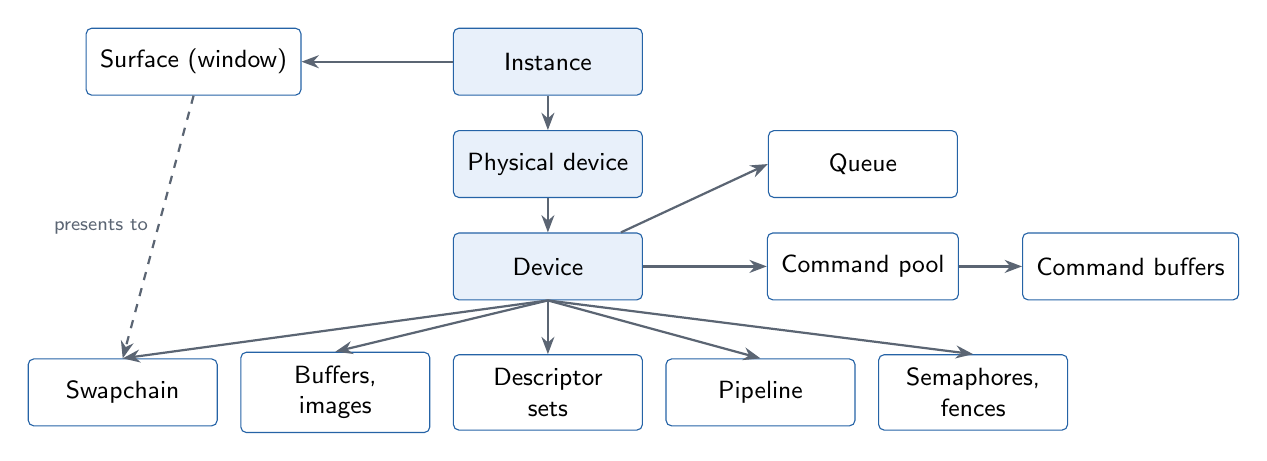
\begin{tikzpicture}[every node/.style={font=\sffamily\scriptsize}, box/.append style={minimum width=2.4cm, minimum height=0.85cm}]
  \node[fillbox] (inst) at (0, 0) {Instance};
  \node[box] (surf) at (-4.5, 0) {Surface (window)};
  \node[fillbox] (phys) at (0, -1.3) {Physical device};
  \node[fillbox] (dev) at (0, -2.6) {Device};
  \node[box] (queue) at (4.0, -1.3) {Queue};
  \node[box] (pool) at (4.0, -2.6) {Command pool};
  \node[box] (cmd) at (7.4, -2.6) {Command buffers};
  \node[box] (mem) at (-2.7, -4.2) {Buffers,\\ images};
  \node[box] (desc) at (0, -4.2) {Descriptor\\ sets};
  \node[box] (pipe) at (2.7, -4.2) {Pipeline};
  \node[box] (sync) at (5.4, -4.2) {Semaphores,\\ fences};
  \node[box] (swap) at (-5.4, -4.2) {Swapchain};
  \draw[arrow] (inst) -- (surf);
  \draw[arrow] (inst) -- (phys);
  \draw[arrow] (phys) -- (dev);
  \draw[arrow] (dev) -- (queue.west);
  \draw[arrow] (dev) -- (pool);
  \draw[arrow] (pool) -- (cmd);
  \foreach \n in {mem,desc,pipe,sync,swap} \draw[arrow] (dev.south) -- (\n.north);
  \draw[arrow, dashed] (surf.south) -- node[label, left] {presents to} (swap.north);
\end{tikzpicture}
\caption{What is created from what. Everything below the device is destroyed before the device.}
\end{figure}

% -----------------------------------------------------------------
\section{VulkanHelpers: the building blocks}

\file{engine/include/VulkanHelpers.h} keeps the rest of the Vulkan code short. Knowing its pieces makes the other classes easy to read.

\subsection{Errors}

Almost every Vulkan function returns a \code{VkResult}. \code{check} turns failure into an exception that names the call:

\begin{lstlisting}
inline void check(VkResult result, const char* what) {
    if (result != VK_SUCCESS) {
        throw std::runtime_error(std::string(what) + " failed (VkResult " + std::to_string(result) + ")");
    }
}
check(vkCreateDevice(m_physicalDevice, &createInfo, nullptr, &m_device), "vkCreateDevice");
\end{lstlisting}

\subsection{Enumerations}

Vulkan returns lists in two calls: one to get the count, one to fill an array. \code{enumerate} does both, for any such function, thanks to a variadic template:

\begin{lstlisting}
template<typename T, typename Function, typename... Args>
[[nodiscard]] std::vector<T> enumerate(Function function, Args... args) {
    uint32_t count = 0;
    function(args..., &count, nullptr);
    std::vector<T> elements(count);
    function(args..., &count, elements.data());
    elements.resize(count);
    return elements;
}
const auto devices = enumerate<VkPhysicalDevice>(vkEnumeratePhysicalDevices, m_instance);
\end{lstlisting}

\subsection{Owning handles}

Vulkan handles are plain values; nothing destroys them for you. \code{DeviceHandle} is a move-only owner, like \code{std::unique_ptr}, that calls the right \code{vkDestroy*} function. The destroy function is a template parameter, so each alias is a distinct type:

\begin{lstlisting}
template<typename Handle, auto Destroy>
class DeviceHandle {
public:
    DeviceHandle(VkDevice device, Handle handle) noexcept : m_device(device), m_handle(handle) {}
    DeviceHandle(DeviceHandle&& other) noexcept;              // takes over the handle
    ~DeviceHandle() { reset(); }                              // Destroy(m_device, m_handle, nullptr)
    [[nodiscard]] Handle get() const noexcept { return m_handle; }
    // ...
};
using UniqueBuffer = DeviceHandle<VkBuffer, vkDestroyBuffer>;
using UniqueFence = DeviceHandle<VkFence, vkDestroyFence>;
using UniquePipeline = DeviceHandle<VkPipeline, vkDestroyPipeline>;
// ... 13 aliases in all
\end{lstlisting}

\subsection{Create-info structs}

Every Vulkan object is created from a \code{Vk*CreateInfo} struct whose first member \code{sType} names the struct. FlyTracer fills them with C++20 \emph{designated initializers}: members you do not name are zero, which is the right default for almost every Vulkan field.

\begin{lstlisting}
const VkFenceCreateInfo createInfo{
    .sType = VK_STRUCTURE_TYPE_FENCE_CREATE_INFO,
    .flags = signaled ? VK_FENCE_CREATE_SIGNALED_BIT : VkFenceCreateFlags{0},
};
\end{lstlisting}

\begin{pitfall}
Designated initializers must follow the declaration order of the struct, so \code{.pNext} comes before \code{.flags}, which comes before the rest. The compiler tells you when the order is wrong.
\end{pitfall}

\subsection{Buffers and images}

\code{Buffer} and \code{Image} bundle a handle, its own memory and (for images) a view. The memory type is chosen with \code{findMemoryType}, which looks for a type allowed by the resource that has the requested properties.

\begin{itemize}
  \item \textbf{Device-local} memory is the fastest for the GPU but the CPU cannot write it directly. Static mesh data and all images live here.
  \item \textbf{Host-visible, host-coherent} memory can be mapped: the CPU writes it with \code{memcpy} and the GPU sees the bytes without an explicit flush. A \code{Buffer} in such memory stays mapped for its whole life.
  \item \code{hostWriteMemoryProperties} asks for memory that is \emph{both} when the GPU has it, as on Apple silicon's unified memory or desktop GPUs with resizable BAR. The per-frame scene buffers use it.
\end{itemize}

\subsection{Submitting work}

\code{submit} wraps \code{vkQueueSubmit2} for one command buffer with an optional wait semaphore, signal semaphore and fence. \code{CommandSubmitter} is for one-time work that the CPU waits for: it records, submits, waits for the queue to go idle, and returns the time that took.

\begin{lstlisting}
VulkanHelpers::CommandSubmitter(device, commandPool, queue).Submit([&](VkCommandBuffer cmd) {
    // record commands; Submit returns after the GPU executed them
});
\end{lstlisting}

\code{StagingUploader} uploads data to device-local memory. Since the CPU cannot write there, each upload is written to a temporary host-visible \emph{staging} buffer, and a copy command moves it to the final buffer. All copies go into one command buffer that is submitted once, in \code{submit()}, after which the staging buffers are freed. \code{uploadTexture} also generates the mip chain by blitting each level into the next, half the size.

\subsection{Barriers}

\code{transitionImageLayout2} records one \code{VkImageMemoryBarrier2}: it moves an image from one layout to another, and it makes the commands after it at \code{dstStage} wait for the commands before it at \code{srcStage}, with the memory written by \code{srcAccess} made visible to \code{dstAccess}. Section~\ref{sec:sync} uses it for every step of a frame.

% -----------------------------------------------------------------
\section{VulkanContext: instance and device}

\file{engine/src/VulkanContext.cpp} creates the objects everything else depends on. Its constructor takes an optional SDL window; without one (benchmark, GPU tests) no surface and no swapchain are created.

\subsection{The instance}

\begin{lstlisting}
const VkApplicationInfo appInfo{
    .sType = VK_STRUCTURE_TYPE_APPLICATION_INFO,
    .pApplicationName = "FlyTracer",
    .pEngineName = "FlyTracer",
    .apiVersion = VK_API_VERSION_1_4,
};
\end{lstlisting}

The instance extensions are the ones SDL needs to make a surface for the window (\code{SDL_Vulkan_GetInstanceExtensions}). In Debug builds the \code{VK_LAYER_KHRONOS_validation} layer is enabled when installed, with a debug messenger that prints warnings and errors in colour. The messenger's create info is also chained into the instance create info (through \code{pNext}), so messages from \code{vkCreateInstance} itself are reported too. Setting \code{FLYTRACER_GPU_VALIDATION=1} additionally turns on GPU-assisted validation, which checks shader accesses at run time.

\subsection{Choosing a GPU}

\code{selectPhysicalDevice} loops over all GPUs and keeps the best one that
\begin{enumerate}
  \item supports Vulkan 1.3 (synchronization2 and dynamic rendering are core there), and
  \item has a queue family that can do graphics \emph{and} compute, and present to the window.
\end{enumerate}
Discrete GPUs score highest, then integrated, virtual and CPU implementations.

\begin{keyidea}[Key idea: one queue]
FlyTracer does all its work (the compute dispatch, the copy to the swapchain, the ImGui draw and presenting) on a single queue. Commands on one queue start in submission order, so with barriers between them there is no need for queue ownership transfers or cross-queue semaphores. A second, async compute queue could overlap work, but would make the synchronization much harder to teach.
\end{keyidea}

\subsection{The logical device and its features}

Vulkan features are off until you enable them. FlyTracer enables exactly what it uses, by chaining feature structs through \code{pNext}:

\begin{lstlisting}
VkPhysicalDeviceVulkan13Features vulkan13Features{
    .sType = VK_STRUCTURE_TYPE_PHYSICAL_DEVICE_VULKAN_1_3_FEATURES,
    .synchronization2 = VK_TRUE,     // vkCmdPipelineBarrier2, vkQueueSubmit2
    .dynamicRendering = VK_TRUE,     // ImGui draws without a render pass
};
VkPhysicalDeviceVulkan12Features vulkan12Features{
    .sType = VK_STRUCTURE_TYPE_PHYSICAL_DEVICE_VULKAN_1_2_FEATURES,
    .pNext = &vulkan13Features,
    .shaderSampledImageArrayNonUniformIndexing = VK_TRUE,  // textures[index] varies per pixel
    .scalarBlockLayout = VK_TRUE,                          // tightly packed buffers
};
const VkDeviceCreateInfo createInfo{
    .sType = VK_STRUCTURE_TYPE_DEVICE_CREATE_INFO,
    .pNext = &vulkan12Features,
    // one queue, and VK_KHR_swapchain when there is a window
};
\end{lstlisting}

Finally the context gets the queue and creates a command pool with \code{VK_COMMAND_POOL_CREATE_RESET_COMMAND_BUFFER_BIT}, so each frame's command buffer can be reset and recorded again.

\begin{pitfall}[Pitfall: enabling everything]
It is tempting to enable every feature the GPU supports. Some, such as \code{robustBufferAccess}, add bounds checks to every memory access and cost performance. Enable what you use.
\end{pitfall}

% -----------------------------------------------------------------
\section{Swapchain}

A window cannot be drawn into directly. The \emph{presentation engine} owns a small set of images; each frame you acquire one, render into it, and hand it back to be shown. \file{engine/src/Swapchain.cpp} makes these choices:

\begin{description}[font=\sffamily\bfseries, leftmargin=0pt]
  \item[Format] \code{B8G8R8A8_UNORM} (or \code{R8G8B8A8_UNORM}) with the sRGB colour space. Deliberately \emph{not} an \code{_SRGB} format: the shader already encodes sRGB itself, and ImGui's colours are sRGB values. An \code{_SRGB} swapchain would encode a second time and wash the image out.
  \item[Present mode] With vsync \code{FIFO}, which waits for the display and is always available; without, \code{MAILBOX} or else \code{IMMEDIATE}.
  \item[Image count] One more than the minimum, so the application rarely waits for the presentation engine to release an image.
  \item[Usage] \code{TRANSFER_DST} (the raytraced image is blitted in) and \code{COLOR_ATTACHMENT} (ImGui draws on top).
  \item[Extent] The surface's current size, or the window size in pixels on platforms that leave it to the application.
\end{description}

For every image the swapchain also creates an image view (for ImGui) and a \emph{render-finished} semaphore. That semaphore belongs to the image rather than to a frame in flight, because a present can still be waiting on it after the frame's fence has signalled; reusing it for the next frame could signal a semaphore that is still in use.

When the window is resized, \code{Recreate} builds a new swapchain, passing the old one as \code{oldSwapchain} so the driver can hand over resources. The caller (\code{VulkanRenderer}) first waits for the GPU to be idle.

% -----------------------------------------------------------------
\section{RaytracingPass: the compute pipeline}

\file{engine/src/RaytracingPass.cpp} owns everything the compute shader needs. It is also used without a window by the benchmark and the GPU tests.

\subsection{Resources}

\begin{center}
\small
\begin{tabularx}{\textwidth}{@{}l l X@{}}
\toprule
\textbf{Resource} & \textbf{Memory} & \textbf{Purpose} \\
\midrule
\code{m_accumulation} & device-local, \code{rgba32f} & Running average of linear radiance, kept between frames \\
\code{m_output} & device-local, \code{rgba8} & Tone-mapped sRGB result, the source of the blit \\
mesh buffers (6) & device-local, uploaded by staging & Vertices, triangles, edges, edge-triangle records, BVH pairs, root pairs \\
\code{m_textures} & device-local, \code{R8G8B8A8_SRGB}, mipmapped & Up to 64; slot 0 is a white $1\times1$ image \\
\code{FrameBuffers} ($\times2$) & host-visible & Materials, spheres, planes, lights, instances, top-level BVH, debug lines \\
descriptor sets ($\times2$) & & One per frame in flight, pointing at that frame's buffers \\
\bottomrule
\end{tabularx}
\end{center}

\subsection{Descriptors and pipeline}

Every binding is a storage buffer except the two storage images and the texture array. The layout is built from the numbers in \file{ShaderInterface.h}:

\begin{lstlisting}
std::array<VkDescriptorSetLayoutBinding, BINDING_COUNT> bindings{};
for (uint32_t binding = 0; binding < BINDING_COUNT; ++binding) {
    bindings[binding] = {binding, VK_DESCRIPTOR_TYPE_STORAGE_BUFFER, 1, VK_SHADER_STAGE_COMPUTE_BIT, nullptr};
}
bindings[BINDING_ACCUMULATION_IMAGE].descriptorType = VK_DESCRIPTOR_TYPE_STORAGE_IMAGE;
bindings[BINDING_OUTPUT_IMAGE].descriptorType = VK_DESCRIPTOR_TYPE_STORAGE_IMAGE;
bindings[BINDING_TEXTURES].descriptorType = VK_DESCRIPTOR_TYPE_COMBINED_IMAGE_SAMPLER;
bindings[BINDING_TEXTURES].descriptorCount = kMaxTextures;
m_descriptorSetLayout = VulkanHelpers::createDescriptorSetLayout(device, bindings);
\end{lstlisting}

A descriptor pool is sized for two sets of that layout, and one set is allocated per frame in flight. The pipeline layout combines the set layout with a push constant range the size of \code{Gpu::PushConstants} (72 bytes, below the 128 bytes Vulkan guarantees). The pipeline itself is created from \code{raytracer.comp.spv}, which CMake compiled with \code{glslc}. A linear, repeating sampler with mipmapping is shared by all textures.

\subsection{Uploading meshes}

\code{UploadMeshes} runs once after the scene's \code{OnInit}, and again from \code{Record} when \code{MeshesChanged} reports added meshes or changed counts or textures. It waits for the GPU to be idle (the old buffers may still be in use), encodes all meshes, uploads the six buffers and the textures with one \code{StagingUploader}, and writes their descriptors into both sets. Textures get $\lfloor\log_2(\max(w,h))\rfloor + 1$ mip levels (\code{std::bit_width}), which the shader uses to pick a sharp but not aliased level per pixel. Unused texture slots point at the white texture, so every descriptor in the array is valid.

\subsection{Per-frame buffers}

The small per-frame buffers grow on demand: when the data no longer fits, a buffer of twice the size is created and its descriptor is rewritten.

\begin{lstlisting}
template<typename T>
void RaytracingPass::writeFrameBuffer(VulkanHelpers::Buffer& buffer, VkDescriptorSet set,
                                      uint32_t binding, const std::vector<T>& data) {
    const VkDeviceSize dataSize = sizeof(T) * data.size();
    if (buffer.buffer() == VK_NULL_HANDLE || buffer.size() < dataSize) {
        const VkDeviceSize capacity = std::max({dataSize, 2 * buffer.size(), VkDeviceSize{sizeof(T)}});
        buffer = VulkanHelpers::Buffer(/* ... */ capacity, VK_BUFFER_USAGE_STORAGE_BUFFER_BIT,
                                       VulkanHelpers::hostWriteMemoryProperties(m_context.PhysicalDevice()));
        VulkanHelpers::writeStorageBufferDescriptor(m_context.Device(), set, binding, buffer.buffer());
    }
    if (dataSize > 0) buffer.write(data.data(), dataSize);
}
\end{lstlisting}

\begin{keyidea}[Key idea: why two copies]
While the GPU executes frame $n$, the CPU already writes the data of frame $n+1$. If both used the same buffer, the CPU could overwrite data the GPU is still reading. With one copy per frame in flight, the CPU only writes a frame's buffers (and replaces its descriptor set's entries) after waiting on that frame's fence, so the GPU is done with them.
\end{keyidea}

\subsection{Recording the dispatch}

\code{Record} is called once per frame with the frame's command buffer:

\begin{enumerate}
  \item Re-upload the meshes if they changed, then \code{EncodeFrame} and write the seven per-frame buffers.
  \item Build the push constants: the camera motor (from \code{CameraMotor}, a motor built from joins of the eye, target and up), the field of view, counts, bounces, exposure.
  \item Decide whether accumulation continues. The bytes of everything that affects the image (materials, primitives, lights, instances and the push constants) are compared with last frame's. If anything changed, \code{sampleIndex} goes back to 0 and the average restarts; otherwise it counts up. Debug lines are drawn after accumulation, so they are left out of the comparison.
  \item Record a barrier on the accumulation image, bind the pipeline and descriptor set, push the constants, and dispatch one invocation per pixel:
\end{enumerate}

\begin{lstlisting}
vkCmdBindPipeline(cmdBuffer, VK_PIPELINE_BIND_POINT_COMPUTE, m_pipeline.get());
vkCmdBindDescriptorSets(cmdBuffer, VK_PIPELINE_BIND_POINT_COMPUTE, m_pipelineLayout.get(),
                        0, 1, &frame.descriptorSet, 0, nullptr);
vkCmdPushConstants(cmdBuffer, m_pipelineLayout.get(), VK_SHADER_STAGE_COMPUTE_BIT, 0,
                   sizeof(pushConstants), &pushConstants);
m_timer.Begin(cmdBuffer, frameIndex);
vkCmdDispatch(cmdBuffer, (extent.width + WORKGROUP_SIZE - 1) / WORKGROUP_SIZE,
              (extent.height + WORKGROUP_SIZE - 1) / WORKGROUP_SIZE, 1);
m_timer.End(cmdBuffer, frameIndex);
\end{lstlisting}

The division rounds up, so the workgroups cover the image even when its size is not a multiple of 8; the shader returns early for invocations outside the image.

% -----------------------------------------------------------------
\section{VulkanRenderer: frames in flight and synchronization}
\label{sec:sync}

\file{engine/src/VulkanRenderer.cpp} ties everything together. It is the place where most Vulkan bugs would show up, so it is worth reading slowly.

\subsection{Frames in flight}

\begin{lstlisting}
struct Frame {
    VkCommandBuffer commandBuffer{VK_NULL_HANDLE};
    VulkanHelpers::UniqueSemaphore imageAvailable;   // signalled when the acquired image is ready
    VulkanHelpers::UniqueFence inFlight;             // signalled when the frame's commands finished
};
std::array<Frame, RaytracingPass::kFramesInFlight> m_frames;   // kFramesInFlight == 2
\end{lstlisting}

With two frames in flight the CPU can prepare frame $n+1$ while the GPU renders frame $n$; neither waits for the other unless one is more than a frame ahead (Figure~\ref{fig:timeline}).

\begin{figure}[h]
\centering
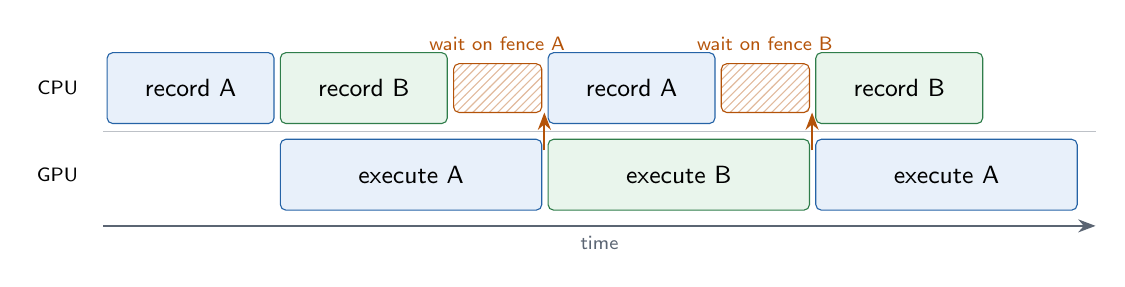
\begin{tikzpicture}[x=1cm, y=1cm, every node/.style={font=\sffamily\scriptsize},
    slot/.style={draw, rounded corners=2pt, minimum height=0.62cm, inner sep=0pt}]
  \newcommand{\slot}[5]{\node[slot, #1, minimum width=#3cm - 0.08cm, anchor=west] at (#2 + 0.04, #4) {#5};}
  \node[anchor=east] at (-0.2, 1.1) {CPU};
  \node[anchor=east] at (-0.2, 0) {GPU};
  \draw[muted!40] (0, 0.55) -- (12.6, 0.55);
  \slot{fillbox}{0}{2.2}{1.1}{record A}
  \slot{greenbox}{2.2}{2.2}{1.1}{record B}
  \slot{fillbox}{2.2}{3.4}{0}{execute A}
  \slot{greenbox}{5.6}{3.4}{0}{execute B}
  \slot{fillbox}{9.0}{3.4}{0}{execute A}
  \node[slot, draw=warm, pattern=north east lines, pattern color=warm!40, minimum width=1.12cm, anchor=west] at (4.44, 1.1) {};
  \node[text=warm, above=1pt] at (5.0, 1.42) {wait on fence A};
  \slot{fillbox}{5.6}{2.2}{1.1}{record A}
  \node[slot, draw=warm, pattern=north east lines, pattern color=warm!40, minimum width=1.12cm, anchor=west] at (7.84, 1.1) {};
  \node[text=warm, above=1pt] at (8.4, 1.42) {wait on fence B};
  \slot{greenbox}{9.0}{2.2}{1.1}{record B}
  \draw[arrow, warm] (5.6, 0.31) -- (5.6, 0.79);
  \draw[arrow, warm] (9.0, 0.31) -- (9.0, 0.79);
  \draw[arrow] (0, -0.65) -- node[label, below] {time} (12.6, -0.65);
\end{tikzpicture}
\caption{Two frames in flight, here with the GPU as the bottleneck. Before the CPU records frame A again it waits on A's fence, while frame B is already queued. The CPU never gets more than two frames ahead.}
\label{fig:timeline}
\end{figure}

\subsection{BeginFrame}

\begin{enumerate}
  \item Skip the frame if the window is minimized (zero pixels); recreate the swapchain if it was marked out of date.
  \item \textbf{Wait on this frame's fence.} After this, the frame's command buffer, per-frame buffers, descriptor set and timestamp queries are free to reuse.
  \item \textbf{Acquire a swapchain image} with \code{vkAcquireNextImageKHR}. It returns an index immediately, but the image may still be read by the display: the \code{imageAvailable} semaphore signals when it really is free. \code{VK_ERROR_OUT_OF_DATE_KHR} means the window changed and the frame is skipped; \code{VK_SUBOPTIMAL_KHR} still renders, but recreates next frame.
  \item If the acquired image was last used by the \emph{other} frame, wait on that frame's fence too (\code{m_imagesInFlight}). This happens when the swapchain returns images out of order.
  \item Reset the fence and start the ImGui frame.
\end{enumerate}

\subsection{EndFrame: one command buffer}

The whole frame is recorded into one command buffer:

\begin{figure}[h]
\centering
\begin{tikzpicture}[node distance=8mm, every node/.style={font=\sffamily\scriptsize},
    stepbox/.style={text width=2.8cm, minimum height=2.0cm}]
  \node[warmbox, stepbox] (dispatch) {\textbf{Dispatch}\\ raytracer.comp\\ writes output};
  \node[fillbox, stepbox, right=of dispatch] (blit) {\textbf{Blit}\\ output $\rightarrow$ swapchain image};
  \node[greenbox, stepbox, right=of blit] (imgui) {\textbf{ImGui}\\ dynamic rendering, loads and stores};
  \node[box, stepbox, right=of imgui] (present) {\textbf{Barrier}\\ to \code{PRESENT_SRC}};
  \draw[arrow] (dispatch) -- (blit); \draw[arrow] (blit) -- (imgui); \draw[arrow] (imgui) -- (present);
  \foreach \n/\t in {dispatch/{output: \texttt{GENERAL}}, blit/{output: \texttt{TRANSFER\_SRC}\\ swapchain: \texttt{TRANSFER\_DST}},
                     imgui/{swapchain: \texttt{COLOR\_ATTACHMENT}}, present/{swapchain: \texttt{PRESENT\_SRC\_KHR}}}
    \node[label, anchor=south, text width=3.2cm] at (\n.center |- 0,1.1) {\t};
\end{tikzpicture}
\caption{The commands of one frame, with the layout of the image each one works on.}
\end{figure}

The compute shader cannot write the swapchain image directly (its format is not guaranteed to support storage), and the raytracer's image is RGBA while the swapchain is usually BGRA. \code{vkCmdBlitImage} copies and converts in one command. Every arrow above is a barrier. The prefixes \code{VK_PIPELINE_STAGE_2_}, \code{VK_ACCESS_2_} and \code{VK_IMAGE_LAYOUT_} are left out in Table~\ref{tab:barriers}.

\begin{table}[h]
\centering
\scriptsize
\renewcommand{\arraystretch}{1.25}
\begin{tabularx}{\textwidth}{@{}l >{\raggedright\arraybackslash}p{1.65cm} >{\raggedright\arraybackslash}p{2.35cm} >{\raggedright\arraybackslash}p{2.45cm} >{\raggedright\arraybackslash}p{2.45cm} >{\raggedright\arraybackslash}X@{}}
\toprule
& \textbf{Image} & \textbf{Layout} & \textbf{Waits for (src)} & \textbf{Before (dst)} & \textbf{Why} \\
\midrule
1 & accumulation & GENERAL $\rightarrow$\newline GENERAL & COMPUTE\_\allowbreak{}SHADER,\newline STORAGE\_\allowbreak{}WRITE & COMPUTE\_\allowbreak{}SHADER,\newline STORAGE\_\allowbreak{}READ|WRITE & The previous frame's dispatch wrote the average this one reads. \\
2 & output & GENERAL $\rightarrow$\newline TRANSFER\_\allowbreak{}SRC & COMPUTE\_\allowbreak{}SHADER,\newline STORAGE\_\allowbreak{}WRITE & BLIT,\newline TRANSFER\_\allowbreak{}READ & The blit reads what the shader wrote. \\
3 & swapchain & UNDEFINED $\rightarrow$\newline TRANSFER\_\allowbreak{}DST & BLIT,\newline NONE & BLIT,\newline TRANSFER\_\allowbreak{}WRITE & Old contents are discarded. The src stage equals the semaphore's wait stage, so the transition happens after the acquire. \\
4 & swapchain & TRANSFER\_\allowbreak{}DST $\rightarrow$\newline COLOR\_\allowbreak{}ATTACHMENT & BLIT,\newline TRANSFER\_\allowbreak{}WRITE & COLOR\_\allowbreak{}ATTACHMENT\_\allowbreak{}OUTPUT,\newline READ|WRITE & ImGui loads the blitted pixels and blends over them. \\
5 & output & TRANSFER\_\allowbreak{}SRC $\rightarrow$\newline GENERAL & BLIT,\newline TRANSFER\_\allowbreak{}READ & COMPUTE\_\allowbreak{}SHADER,\newline STORAGE\_\allowbreak{}WRITE & The next dispatch may only overwrite the output after the blit read it. \\
6 & swapchain & COLOR\_\allowbreak{}ATTACHMENT $\rightarrow$\newline PRESENT\_\allowbreak{}SRC & COLOR\_\allowbreak{}ATTACHMENT\_\allowbreak{}OUTPUT,\newline WRITE & NONE & The presentation engine needs \code{PRESENT_SRC}; the semaphore makes the writes available. \\
\bottomrule
\end{tabularx}
\caption{The barriers of one frame, in recording order (1 is in \texttt{RaytracingPass::Record}, 2--5 in \texttt{recordBlitToSwapchain}, 6 in \texttt{EndFrame}).}
\label{tab:barriers}
\end{table}

\subsection{Submit and present}

\begin{lstlisting}
const VkSemaphoreSubmitInfo waitInfo{
    .sType = VK_STRUCTURE_TYPE_SEMAPHORE_SUBMIT_INFO,
    .semaphore = frame.imageAvailable.get(),
    .stageMask = VK_PIPELINE_STAGE_2_BLIT_BIT,          // only the blit has to wait for the image
};
const VkSemaphoreSubmitInfo signalInfo{
    .sType = VK_STRUCTURE_TYPE_SEMAPHORE_SUBMIT_INFO,
    .semaphore = renderFinished,                          // of this swapchain image
    .stageMask = VK_PIPELINE_STAGE_2_ALL_COMMANDS_BIT,   // includes the transition to PRESENT_SRC
};
VulkanHelpers::submit(m_context.Queue(), cmdBuffer, &waitInfo, &signalInfo, frame.inFlight.get());
\end{lstlisting}

Three synchronization objects work together:

\begin{itemize}
  \item \code{imageAvailable}: presentation engine $\rightarrow$ GPU. The wait stage is \code{BLIT}, not the top of the pipe, so the raytracing dispatch runs while the display still shows the image; only the blit waits.
  \item \code{renderFinished}: GPU $\rightarrow$ presentation engine. \code{vkQueuePresentKHR} waits on it.
  \item \code{inFlight} fence: GPU $\rightarrow$ CPU. \code{BeginFrame} waits on it the next time this frame comes round.
\end{itemize}

When present returns \code{OUT_OF_DATE} or \code{SUBOPTIMAL}, or the window reports a resize, the swapchain is marked outdated. The next \code{BeginFrame} waits for the GPU to be idle and recreates the swapchain, tells ImGui the new image count, and resizes the raytracer's images (which restarts accumulation).

\begin{tryit}[Try it: check the synchronization]
Build Debug and run \code{VK_LAYER_VALIDATE_SYNC=1 ./build-debug/bin/FlyTracer}. The validation layer then tracks every access to every image and buffer and reports hazards such as a write after read without a barrier. A correct frame prints nothing. As an exercise, work out which hazard each barrier in Table~\ref{tab:barriers} prevents, then remove one and see what the layer says.
\end{tryit}

% -----------------------------------------------------------------
\section{ImGui with dynamic rendering}

Dear ImGui draws triangles with a graphics pipeline, which needs a colour attachment. Classic Vulkan required a \code{VkRenderPass} and a \code{VkFramebuffer} per swapchain image for that, both recreated on every resize. Since Vulkan 1.3, \emph{dynamic rendering} replaces them with one call that names the attachment directly:

\begin{lstlisting}
const VkRenderingAttachmentInfo colorAttachment{
    .sType = VK_STRUCTURE_TYPE_RENDERING_ATTACHMENT_INFO,
    .imageView = view,                                         // the swapchain image's view
    .imageLayout = VK_IMAGE_LAYOUT_COLOR_ATTACHMENT_OPTIMAL,
    .loadOp = VK_ATTACHMENT_LOAD_OP_LOAD,                      // keep the raytraced image
    .storeOp = VK_ATTACHMENT_STORE_OP_STORE,
};
const VkRenderingInfo renderingInfo{
    .sType = VK_STRUCTURE_TYPE_RENDERING_INFO,
    .renderArea = {{0, 0}, extent},
    .layerCount = 1,
    .colorAttachmentCount = 1,
    .pColorAttachments = &colorAttachment,
};
vkCmdBeginRendering(cmdBuffer, &renderingInfo);
ImGui_ImplVulkan_RenderDrawData(ImGui::GetDrawData(), cmdBuffer);
vkCmdEndRendering(cmdBuffer);
\end{lstlisting}

\code{LOAD_OP_LOAD} is essential: \code{CLEAR} or \code{DONT_CARE} would throw away the raytraced pixels under the UI. At initialization ImGui is told the swapchain's colour format (\code{UseDynamicRendering} with a \code{VkPipelineRenderingCreateInfo}), so it can build its pipeline without a render pass. Because ImGui keeps a pointer to that format, \code{ImGuiLayer} stores it in a member that lives as long as ImGui does.

% -----------------------------------------------------------------
\section{Measuring: GpuTimer and Benchmark}

\code{GpuTimer} writes a timestamp before and after the dispatch into a query pool (two queries per frame in flight). The results are read back when the frame's slot is reused, after its fence: reading earlier would stall the CPU. Some drivers resolve all timestamps of a command buffer to the same value (KosmicKrisp on macOS does); the timer then reports nothing and the GUI says ``not measurable with this driver''.

The benchmark (\code{--benchmark 200}) needs no window. It creates a headless \code{VulkanContext} and a \code{RaytracingPass}, and for each scene advances the scene with a fixed time step, records the dispatch with a \code{CommandSubmitter} and measures the time from submit to completion. An empty submission is measured first, so you can tell how much of a frame is overhead. Compare at 1080p or more: small images are dominated by that overhead.

% ================================================================= PART III
\partheading{III}{The GPU Side}

\section{The compute shader}

\subsection{Files}

\begin{center}
\small
\begin{tabularx}{\textwidth}{@{}>{\sffamily}l X@{}}
\toprule
\textbf{File} & \textbf{Contents} \\
\midrule
raytracer.comp & \code{main}: the camera ray, the bounce loop, accumulation and output \\
flyfish.glsl & FlyFish's types and products in GLSL, same coefficients and signs: join, meet, inner, geometric product, sandwich \\
common.glsl, bindings.glsl & GPU structs (matching \file{GpuScene.h}), descriptor bindings and push constants \\
ray.glsl & The ray: a point and a direction, and where a ray meets a plane \\
intersections.glsl & Ray tests for spheres, planes and boxes; the watertight Plücker test for triangle edges \\
traversal.glsl & The two-level BVH traversal \\
brdf.glsl, shading.glsl & Sky, BRDFs (Lambert, Blinn-Phong, Cook-Torrance), lights, shadow rays, reflections \\
random.glsl, output.glsl, debug\_lines.glsl & Random numbers, ACES tone mapping and sRGB encoding, the debug line overlay \\
\bottomrule
\end{tabularx}
\end{center}

\subsection{One invocation per pixel}

\begin{lstlisting}[style=glsl]
layout(local_size_x = WORKGROUP_SIZE, local_size_y = WORKGROUP_SIZE) in;

void main() {
    ivec2 pixel = ivec2(gl_GlobalInvocationID.xy);
    ivec2 size = imageSize(outputImage);
    if (pixel.x >= size.x || pixel.y >= size.y) return;

    // The first sample goes through the pixel center, later ones are spread over the pixel
    uint rng = seedRandom(pixel, pc.frameIndex);
    vec2 jitter = pc.sampleIndex == 0u ? vec2(0.5) : vec2(random(rng), random(rng));
    // ...
    vec3 radiance = traceRadiance(cameraRay(vec2(pixel) + jitter, vec2(size)), pixelAngle, rng, hitDistance);

    // Running average of all samples since the view or scene last changed
    vec3 average = radiance;
    if (pc.sampleIndex > 0u) {
        vec3 previous = imageLoad(accumulationImage, pixel).rgb;
        average = previous + (radiance - previous) / float(pc.sampleIndex + 1u);
    }
    imageStore(accumulationImage, pixel, vec4(average, 1.0));

    vec3 color = toneMapACES(average * pc.exposure);
    color = drawDebugLines(cameraRay(vec2(pixel) + 0.5, vec2(size)), hitDistance, pixelAngle, color);
    imageStore(outputImage, pixel, vec4(linearToSrgb(color), 1.0));
}
\end{lstlisting}

The running average is the reason a still image becomes smooth after a moment: every frame adds one jittered sample per pixel, which anti-aliases edges and averages the noise of glossy reflections. This is also why \code{RaytracingPass} must notice when anything changes and reset \code{sampleIndex}: otherwise a moving object would leave a trail.

\subsection{The camera is a motor}

\begin{lstlisting}[style=glsl]
Ray cameraRay(vec2 pixel, vec2 imageSize) {
    vec2 ndc = 2.0 * pixel / imageSize - 1.0;
    float aspect = imageSize.x / imageSize.y;
    Motor camera = Motor(pc.cameraRotor.x, pc.cameraRotor.yzw, pc.cameraDual.xyz, pc.cameraDual.w);
    TriVector towards = direction(vec3(ndc.x * aspect * pc.tanHalfFov, -ndc.y * pc.tanHalfFov, -1.0));
    return Ray(sandwich(camera, point(vec3(0.0))), normalized(sandwich(camera, towards)));
}
\end{lstlisting}

In the camera's own frame every ray starts at the origin and looks down $-z$. The camera motor, built on the CPU from joins of eye, target and up, moves the origin and the direction into the world with the same sandwich $M\,X\,\widetilde{M}$ the C++ side uses. No view matrix exists anywhere.

\subsection{Rays into instances}

To test a ray against an instance, the shader moves the \emph{ray} into the mesh's object space instead of moving the mesh into the world: undo the mirror (a reflection is its own inverse), sandwich with the reversed motor, divide by the scale. The direction is not renormalized, so a distance $t$ along the ray means the same in both spaces and hits from different instances can be compared directly.

\begin{lstlisting}[style=glsl]
Ray toObjectSpace(Ray ray, MeshInstance instance) {
    if (instance.hasMirror != 0u) {
        Vector mirror = Vector(instance.mirror.xyz, instance.mirror.w);
        ray = Ray(reflectInPlane(mirror, ray.origin), reflectInPlane(mirror, ray.direction));
    }
    Motor toObject = reverse(instanceMotor(instance));
    TriVector origin = sandwich(toObject, ray.origin);
    TriVector towards = sandwich(toObject, ray.direction);
    return Ray(point(origin.xyz / instance.scale), direction(towards.xyz / instance.scale));
}
\end{lstlisting}

Traversal keeps a small stack of node pairs with the distance at which the ray enters them. Pairs entered beyond the closest hit so far are skipped, and the nearer child is visited first, so most of the tree is never touched. Shadow rays use the same traversal in \emph{any-hit} mode, which stops at the first hit.

% -----------------------------------------------------------------
\section{Testing and debugging}

\begin{center}
\small
\begin{tabularx}{\textwidth}{@{}>{\sffamily}l X l@{}}
\toprule
\textbf{Executable} & \textbf{Tests} & \textbf{GPU} \\
\midrule
FlyTracer\_Test & BVH, PGA helpers, camera, input, GPU encoding, meshes, scene encoding & no \\
FlyTracer\_ConfigTest & The config file parser & no \\
FlyTracer\_ShaderTest & \file{flyfish.glsl} against FlyFish; GLSL struct layouts, bindings and push constants against \file{GpuScene.h} & yes \\
FlyTracer\_SceneTest & A golden image of every registered scene & yes \\
FlyTracer\_RenderTest & A golden image of a test scene, and the benchmark & yes \\
\bottomrule
\end{tabularx}
\end{center}

Golden image tests render a scene headless and compare it with a reference image in \file{tests/reference}. When a reference is missing it is recorded, so after an intended change in the look you delete the reference and run the test again.

For Vulkan problems, three tools in increasing order of effort:

\begin{enumerate}
  \item A \textbf{Debug build} enables the validation layer: wrong parameters, missing features and leaked objects are reported immediately, with the name of the rule that was broken.
  \item \code{VK_LAYER_VALIDATE_SYNC=1} adds synchronization validation (missing or wrong barriers).
  \item \code{FLYTRACER_GPU_VALIDATION=1} adds GPU-assisted validation, which instruments the shader to catch out-of-bounds buffer and descriptor accesses.
\end{enumerate}

\begin{pitfall}[Pitfall: stale shaders]
Shaders are compiled by the build. When you edit a GLSL file, rebuild before you run, or you test the old SPIR-V. A shader that fails to compile fails the build, with \code{glslc}'s message pointing at the line.
\end{pitfall}

% -----------------------------------------------------------------
\section{Exercises}

\begin{enumerate}[leftmargin=1.5em, itemsep=6pt]
  \item \textbf{A spinning scene.} Write a scene with a mesh that turns about a line that does not pass through the origin. Build the line as the join of two points and the motor with \code{Motor::Rotation}. Draw the line with \code{DrawDebugLine}.
  \item \textbf{Follow a frame.} Set breakpoints in \code{BeginFrame}, \code{RaytracingPass::Record} and \code{EndFrame}. In which order are the fence wait, the acquire, the encoding and the submit executed? Where would the CPU block if the GPU were slow?
  \item \textbf{Workgroup size.} Change \code{WORKGROUP_SIZE} in \file{ShaderInterface.h} to 4 and to 16 and run the benchmark at 1080p. Why does one header change both the C++ dispatch and the shader?
  \item \textbf{Present modes.} Run with and without \code{--no-vsync} and compare the printed swapchain line and the frame rate. What does \code{MAILBOX} do differently from \code{FIFO}?
  \item \textbf{Three frames in flight.} What has to change for \code{kFramesInFlight = 3}? Check the descriptor pool sizes, \code{FrameBuffers}, \code{GpuTimer} and the benchmark's \code{firstMeasured}.
  \item \textbf{A new per-frame buffer.} Add a binding to \file{ShaderInterface.h}, a struct with \code{static_assert}s to \file{GpuScene.h} and its twin to \file{common.glsl}, a buffer to \file{bindings.glsl}, a vector to \code{FrameData}, and one \code{writeFrameBuffer} call. Then run \code{FlyTracer_ShaderTest}: does it catch a mismatch you introduce on purpose?
\end{enumerate}

% -----------------------------------------------------------------
\appendix
\section{Vulkan calls by class}

Every Vulkan function the engine calls, grouped by where it is called. The \code{vkDestroy*} functions are called by the \code{DeviceHandle} aliases.

\begin{center}
\small
\begin{tabularx}{\textwidth}{@{}>{\sffamily\raggedright\arraybackslash}p{3.1cm} >{\raggedright\arraybackslash}X@{}}
\toprule
\textbf{Where} & \textbf{Calls} \\
\midrule
VulkanContext & \code{vkCreateInstance}, \code{vkEnumerateInstanceLayerProperties}, \code{vkCreateDebugUtilsMessengerEXT}, \code{vkEnumeratePhysicalDevices}, \code{vkGetPhysicalDeviceProperties}, \code{vkGetPhysicalDeviceQueueFamilyProperties}, \code{vkGetPhysicalDeviceSurfaceSupportKHR}, \code{vkCreateDevice}, \code{vkGetDeviceQueue}, \code{vkCreateCommandPool}, \code{vkDeviceWaitIdle} \\
Swapchain & \code{vkGetPhysicalDeviceSurfaceCapabilitiesKHR}, \code{vkGetPhysicalDeviceSurfaceFormatsKHR}, \code{vkGetPhysicalDeviceSurfacePresentModesKHR}, \code{vkCreateSwapchainKHR}, \code{vkGetSwapchainImagesKHR} \\
VulkanHelpers & \code{vkCreateBuffer}, \code{vkCreateImage}, \code{vkCreateImageView}, \code{vkGetBufferMemoryRequirements}, \code{vkGetImageMemoryRequirements}, \code{vkGetPhysicalDeviceMemoryProperties}, \code{vkAllocateMemory}, \code{vkBindBufferMemory}, \code{vkBindImageMemory}, \code{vkMapMemory}, \code{vkCreateSemaphore}, \code{vkCreateFence}, \code{vkCreateDescriptorSetLayout}, \code{vkCreateDescriptorPool}, \code{vkAllocateDescriptorSets}, \code{vkUpdateDescriptorSets}, \code{vkCreatePipelineLayout}, \code{vkCreateShaderModule}, \code{vkCreateComputePipelines}, \code{vkAllocateCommandBuffers}, \code{vkResetCommandBuffer}, \code{vkBeginCommandBuffer}, \code{vkEndCommandBuffer}, \code{vkQueueSubmit2}, \code{vkQueueWaitIdle}, \code{vkFreeCommandBuffers}, \code{vkCmdPipelineBarrier2}, \code{vkCmdCopyBuffer}, \code{vkCmdCopyBufferToImage}, \code{vkCmdBlitImage} \\
RaytracingPass & \code{vkCreateSampler}, \code{vkCmdBindPipeline}, \code{vkCmdBindDescriptorSets}, \code{vkCmdPushConstants}, \code{vkCmdDispatch} \\
VulkanRenderer & \code{vkWaitForFences}, \code{vkResetFences}, \code{vkAcquireNextImageKHR}, \code{vkCmdBlitImage}, \code{vkQueuePresentKHR} \\
ImGuiLayer & \code{vkCmdBeginRendering}, \code{vkCmdEndRendering} (the rest is inside \code{imgui_impl_vulkan}) \\
GpuTimer & \code{vkCreateQueryPool}, \code{vkCmdResetQueryPool}, \code{vkCmdWriteTimestamp2}, \code{vkGetQueryPoolResults} \\
\bottomrule
\end{tabularx}
\end{center}

\section{Further reading}

\begin{itemize}
  \item \file{docs/pga-tracer.md}: the mathematics of the tracer (camera, rays, triangles, instances, shading) in more depth.
  \item \file{docs/scenes/}: the student guide to writing scenes.
  \item The Vulkan specification, chapter ``Synchronization and Cache Control'', for the exact meaning of stages and access masks.
  \item S.~De~Keninck et al., ``Clean up your Mesh!'' (2025), for the mesh measures in \code{Mesh}.
\end{itemize}

\end{document}
